% Options for packages loaded elsewhere
\PassOptionsToPackage{unicode}{hyperref}
\PassOptionsToPackage{hyphens}{url}
%
\documentclass[
  ignorenonframetext,
]{beamer}
\usepackage{pgfpages}
\setbeamertemplate{caption}[numbered]
\setbeamertemplate{caption label separator}{: }
\setbeamercolor{caption name}{fg=normal text.fg}
\beamertemplatenavigationsymbolsempty
% Prevent slide breaks in the middle of a paragraph
\widowpenalties 1 10000
\raggedbottom
\setbeamertemplate{part page}{
  \centering
  \begin{beamercolorbox}[sep=16pt,center]{part title}
    \usebeamerfont{part title}\insertpart\par
  \end{beamercolorbox}
}
\setbeamertemplate{section page}{
  \centering
  \begin{beamercolorbox}[sep=12pt,center]{section title}
    \usebeamerfont{section title}\insertsection\par
  \end{beamercolorbox}
}
\setbeamertemplate{subsection page}{
  \centering
  \begin{beamercolorbox}[sep=8pt,center]{subsection title}
    \usebeamerfont{subsection title}\insertsubsection\par
  \end{beamercolorbox}
}
\AtBeginPart{
  \frame{\partpage}
}
\AtBeginSection{
  \ifbibliography
  \else
    \frame{\sectionpage}
  \fi
}
\AtBeginSubsection{
  \frame{\subsectionpage}
}
\usepackage{amsmath,amssymb}
\usepackage{iftex}
\ifPDFTeX
  \usepackage[T1]{fontenc}
  \usepackage[utf8]{inputenc}
  \usepackage{textcomp} % provide euro and other symbols
\else % if luatex or xetex
  \usepackage{unicode-math} % this also loads fontspec
  \defaultfontfeatures{Scale=MatchLowercase}
  \defaultfontfeatures[\rmfamily]{Ligatures=TeX,Scale=1}
\fi
\usepackage{lmodern}
\ifPDFTeX\else
  % xetex/luatex font selection
\fi
% Use upquote if available, for straight quotes in verbatim environments
\IfFileExists{upquote.sty}{\usepackage{upquote}}{}
\IfFileExists{microtype.sty}{% use microtype if available
  \usepackage[]{microtype}
  \UseMicrotypeSet[protrusion]{basicmath} % disable protrusion for tt fonts
}{}
\makeatletter
\@ifundefined{KOMAClassName}{% if non-KOMA class
  \IfFileExists{parskip.sty}{%
    \usepackage{parskip}
  }{% else
    \setlength{\parindent}{0pt}
    \setlength{\parskip}{6pt plus 2pt minus 1pt}}
}{% if KOMA class
  \KOMAoptions{parskip=half}}
\makeatother
\usepackage{xcolor}
\newif\ifbibliography
\usepackage{color}
\usepackage{fancyvrb}
\newcommand{\VerbBar}{|}
\newcommand{\VERB}{\Verb[commandchars=\\\{\}]}
\DefineVerbatimEnvironment{Highlighting}{Verbatim}{commandchars=\\\{\}}
% Add ',fontsize=\small' for more characters per line
\usepackage{framed}
\definecolor{shadecolor}{RGB}{248,248,248}
\newenvironment{Shaded}{\begin{snugshade}}{\end{snugshade}}
\newcommand{\AlertTok}[1]{\textcolor[rgb]{0.94,0.16,0.16}{#1}}
\newcommand{\AnnotationTok}[1]{\textcolor[rgb]{0.56,0.35,0.01}{\textbf{\textit{#1}}}}
\newcommand{\AttributeTok}[1]{\textcolor[rgb]{0.13,0.29,0.53}{#1}}
\newcommand{\BaseNTok}[1]{\textcolor[rgb]{0.00,0.00,0.81}{#1}}
\newcommand{\BuiltInTok}[1]{#1}
\newcommand{\CharTok}[1]{\textcolor[rgb]{0.31,0.60,0.02}{#1}}
\newcommand{\CommentTok}[1]{\textcolor[rgb]{0.56,0.35,0.01}{\textit{#1}}}
\newcommand{\CommentVarTok}[1]{\textcolor[rgb]{0.56,0.35,0.01}{\textbf{\textit{#1}}}}
\newcommand{\ConstantTok}[1]{\textcolor[rgb]{0.56,0.35,0.01}{#1}}
\newcommand{\ControlFlowTok}[1]{\textcolor[rgb]{0.13,0.29,0.53}{\textbf{#1}}}
\newcommand{\DataTypeTok}[1]{\textcolor[rgb]{0.13,0.29,0.53}{#1}}
\newcommand{\DecValTok}[1]{\textcolor[rgb]{0.00,0.00,0.81}{#1}}
\newcommand{\DocumentationTok}[1]{\textcolor[rgb]{0.56,0.35,0.01}{\textbf{\textit{#1}}}}
\newcommand{\ErrorTok}[1]{\textcolor[rgb]{0.64,0.00,0.00}{\textbf{#1}}}
\newcommand{\ExtensionTok}[1]{#1}
\newcommand{\FloatTok}[1]{\textcolor[rgb]{0.00,0.00,0.81}{#1}}
\newcommand{\FunctionTok}[1]{\textcolor[rgb]{0.13,0.29,0.53}{\textbf{#1}}}
\newcommand{\ImportTok}[1]{#1}
\newcommand{\InformationTok}[1]{\textcolor[rgb]{0.56,0.35,0.01}{\textbf{\textit{#1}}}}
\newcommand{\KeywordTok}[1]{\textcolor[rgb]{0.13,0.29,0.53}{\textbf{#1}}}
\newcommand{\NormalTok}[1]{#1}
\newcommand{\OperatorTok}[1]{\textcolor[rgb]{0.81,0.36,0.00}{\textbf{#1}}}
\newcommand{\OtherTok}[1]{\textcolor[rgb]{0.56,0.35,0.01}{#1}}
\newcommand{\PreprocessorTok}[1]{\textcolor[rgb]{0.56,0.35,0.01}{\textit{#1}}}
\newcommand{\RegionMarkerTok}[1]{#1}
\newcommand{\SpecialCharTok}[1]{\textcolor[rgb]{0.81,0.36,0.00}{\textbf{#1}}}
\newcommand{\SpecialStringTok}[1]{\textcolor[rgb]{0.31,0.60,0.02}{#1}}
\newcommand{\StringTok}[1]{\textcolor[rgb]{0.31,0.60,0.02}{#1}}
\newcommand{\VariableTok}[1]{\textcolor[rgb]{0.00,0.00,0.00}{#1}}
\newcommand{\VerbatimStringTok}[1]{\textcolor[rgb]{0.31,0.60,0.02}{#1}}
\newcommand{\WarningTok}[1]{\textcolor[rgb]{0.56,0.35,0.01}{\textbf{\textit{#1}}}}
\usepackage{graphicx}
\makeatletter
\newsavebox\pandoc@box
\newcommand*\pandocbounded[1]{% scales image to fit in text height/width
  \sbox\pandoc@box{#1}%
  \Gscale@div\@tempa{\textheight}{\dimexpr\ht\pandoc@box+\dp\pandoc@box\relax}%
  \Gscale@div\@tempb{\linewidth}{\wd\pandoc@box}%
  \ifdim\@tempb\p@<\@tempa\p@\let\@tempa\@tempb\fi% select the smaller of both
  \ifdim\@tempa\p@<\p@\scalebox{\@tempa}{\usebox\pandoc@box}%
  \else\usebox{\pandoc@box}%
  \fi%
}
% Set default figure placement to htbp
\def\fps@figure{htbp}
\makeatother
\setlength{\emergencystretch}{3em} % prevent overfull lines
\providecommand{\tightlist}{%
  \setlength{\itemsep}{0pt}\setlength{\parskip}{0pt}}
\setcounter{secnumdepth}{-\maxdimen} % remove section numbering
\usepackage{bookmark}
\IfFileExists{xurl.sty}{\usepackage{xurl}}{} % add URL line breaks if available
\urlstyle{same}
\hypersetup{
  pdftitle={Module 1: INTRODUCTION},
  pdfauthor={Bob O'Hara, Department of Mathematical Sciences, NTNU},
  hidelinks,
  pdfcreator={LaTeX via pandoc}}

\title{Module 1: INTRODUCTION}
\subtitle{TMA4315 Generalized linear models H2025}
\author{Bob O'Hara, Department of Mathematical Sciences, NTNU}
\date{18.08 {[}PL{]} and 20.08 {[}IL{]}}

\begin{document}
\frame{\titlepage}

\begin{frame}{Introduction: Links}
\phantomsection\label{introduction-links}
Course: \url{https://www.ntnu.edu/studies/courses/TMA4315\#tab=omEmnet}

Wiki: \url{https://wiki.math.ntnu.no/tma4315/2025h/start}

GitHub: \url{https://github.com/oharar/TMA4315}


\includegraphics[width=\linewidth,height=0.4\textheight,keepaspectratio]{WikiTMA4315_2025.png}
\end{frame}

\begin{frame}{Introduction: Aim of this module}
\phantomsection\label{introduction-aim-of-this-module}
\begin{itemize}
\item
  Introduction (to the introduction\ldots)
\item
  What we will teach
\item
  How we will teach
\item
  Where we are going with GLMs
\item
  short presentation of all course modules
\item
  learning outcomes
\item
  student learning styles
\item
  interactive lectures: what, why and how?
\item
  practical details of the course (Blackboard)
\end{itemize}
\end{frame}

\begin{frame}[fragile]{Introduction: Aim of this module}
\phantomsection\label{introduction-aim-of-this-module-1}
\begin{itemize}
\tightlist
\item
  core concept: the exponential family of distributions
\item
  learn about - and use - \texttt{R}, \texttt{Rstudio},
  \texttt{R\ Markdown}, and get familiar with related topics
\item
  get up to speed on R (and writing reports in R markdown) to be able to
  do the 3*10-points compulsory exercises by doing recommended exercises
\end{itemize}
\end{frame}

\begin{frame}
\begin{block}{Where we are going with GLMs: Expanding the linear
regression framework}
\phantomsection\label{where-we-are-going-with-glms-expanding-the-linear-regression-framework}
We will stay with regression (for the whole course) - but make
expansions in several directions.

What will not change:

\begin{itemize}
\item
  our target is \emph{a random response \(Y_i\)} (from some statistical
  distribution): continuous, binary, nominal or ordinal, we have
\item
  \emph{fixed covariates (or explanatory variables) \(X_i\)} (in a
  design matrix): quantitative or qualitative, and
\item
  \emph{unknown regression parameters \(\beta\)}.
\end{itemize}
\end{block}
\end{frame}

\begin{frame}
\begin{block}{Expanding the linear regression framework}
\phantomsection\label{expanding-the-linear-regression-framework}
We will consider relationships between the \emph{conditional mean of
\(Y_i\)}, \(\text{E}(Y_i\mid {\bf x}_i)=\mu_i\), and linear combinations
of the covariates in \emph{a linear predictor}

\[
\eta_i=\beta_0+\beta_1 x_{i1}+\cdots +\beta_k x_{ik}={\bf x}_i^T \boldsymbol{\beta}.
\]

We connect \(\eta_i\) and \(\mu\) through a \emph{link function}:
\[\mu_i = g^{-1}(\eta_i)\]
\end{block}
\end{frame}

\begin{frame}
\begin{block}{Expanding the linear regression framework even more}
\phantomsection\label{expanding-the-linear-regression-framework-even-more}
For most of the course we will assume observation pairs
(\(Y_i,{\bf x}_i\)) are independent \(i=1,\ldots,n\), but we will also
consider clustered pairs (in Module 7+8: Linear mixed effects models LMM
and Generalized linear mixed effects models GLMM).

\[
\eta_i={\bf x}_i^T \boldsymbol{\beta} + \bf{Z} u
\]

(notation to be explained: the take-home message is that this is still
linear)
\end{block}
\end{frame}

\begin{frame}
\begin{block}{Modules}
\phantomsection\label{modules}
The course is split up into 9 modules, which take 1-2 weeks of class.

Each module has a different theme
\end{block}
\end{frame}

\begin{frame}
\begin{block}{The modules - in short}
\phantomsection\label{the-modules---in-short}
The modules of this course are:

\begin{enumerate}
\item
  Introduction (the module page you are reading now) {[}week 34{]}
\item
  Multiple linear regression (emphasis on likelihood) {[}week 35-36{]}
\item
  Binary regression (binary individual and grouped response) {[}week
  37-38{]}
\item
  Poisson and gamma regression (count, non-normal continuous) {[}week
  39-40{]}
\item
  GLM in general and quasi likelihood (exponential family, link
  function) {[}week 41{]}
\item
  Categorical regression and contingency tables {[}week 43{]}
\item
  Linear mixed models (clustered data, repeated measurements) {[}week
  44-45{]}
\item
  Generalized mixed effects models {[}week 46{]}
\item
  Discussion and conclusion {[}week 47{]}
\end{enumerate}
\end{block}
\end{frame}

\begin{frame}
\begin{block}{Common - for all modules}
\phantomsection\label{common---for-all-modules}
\begin{enumerate}
\item
  Model specification: an equation linking the response and the
  explanatory variables, and a probability distribution for the
  response.
\item
  Estimation of the parameters in the model
\item
  Checking the adequacy of the model, how well it fits the data.
\item
  Inference: confidence intervals, hypothesis tests, interpretation of
  results, prediction of future responses.
\end{enumerate}

Both theoretic derivations and practical analysis in R will be
emphasized.
\end{block}
\end{frame}

\begin{frame}[fragile]
\begin{block}{Module 2: Multiple linear regression}
\phantomsection\label{module-2-multiple-linear-regression}
\textbf{PLAN:} You recapitulate what you have learned in TMA4267 Linear
statistical models (or an equivalent course!), and in the plenary
lectures we focus on a three-step model, likelihood theory and formal
inference connected to the likelihood. Instead of sums-of-squares of
error (MSE, RSS) we will use deviance.

In Compulsory exercise 1 you make your own \texttt{mylm} function to
perform MLR.

\textbf{Textbook}: Chapter 3 (from TMA4267) and parts of Appendix B4.
\end{block}
\end{frame}

\begin{frame}
\begin{block}{Module 3: Binary regression}
\phantomsection\label{module-3-binary-regression}
How can be model a response that is not a continuous variable? Here we
look at present/absent, true/false, healthy/diseased.

\textbf{PLAN:} In this module we will study the binary regression, work
on parameter estimation and interpretation of parameter estimates using
odds, work with both individual and grouped data, test linear
hypotheses, look at criteria for model fit and model choice, and discuss
overdispersion.

\textbf{Textbook:} 2.3 and 5.1.
\end{block}
\end{frame}

\begin{frame}
\begin{block}{Module 4: Poisson and gamma regression}
\phantomsection\label{module-4-poisson-and-gamma-regression}
Count data - the number of times and event occurs - is common.

Continuous positive data - like life times, costs and claim sized

\textbf{Plan} We will look at effect a one of more covariates that may
work multiplicative on the response and see how we may fit that assuming
a Poisson distribution (counts) or gamma regression (continuous) on the
log scale of the response.

\textbf{Textbook:} 5.2 and 5.3
\end{block}
\end{frame}

\begin{frame}
\begin{block}{Module 5: GLM in general (and quasi likelihood --- if
time)}
\phantomsection\label{module-5-glm-in-general-and-quasi-likelihood-if-time}
We will see that normal, binary, Poisson and gamma regression all have
the same underlying features: this leads to a unified framework, and
maximum likelihood estimation can be written on a generalized form for
all GLMs

\textbf{Plan} Develop the maths for GLMs, including their statistical
inference and asymptotic properties of estimators on a common form.
Finally, we may expand this to quasi-likelihood models by just
specifying mean and variance (not distribution).

This part is rather mathematical - but is built on the findings of
modules 1-4.

\textbf{Textbook:} 5.4 and 5.5
\end{block}
\end{frame}

\begin{frame}
\begin{block}{Module 6: Categorical regression and contingency tables}
\phantomsection\label{module-6-categorical-regression-and-contingency-tables}
Here our response variable has more than two categories, and these
categories can either be unordered or ordered.

\textbf{Plan} We will use the multinomial distribution as the
distribution for the response, and work mainly with grouped data - that
often can be presented in a contingency table. For ordered categories
(like the defoliation of trees) we will use a cumulative model, also
called a proportional odds model.

\textbf{Textbook:} Chapter 6, and possibly extra material on the Fisher
and Chi-square test (if time permits).

Compulsory exercise 2 will cover modules 3-6.
\end{block}
\end{frame}

\begin{frame}
\begin{block}{Module 7: Linear mixed effects models}
\phantomsection\label{module-7-linear-mixed-effects-models}
We sometimes have categorical factors with lots of levels, e.g.~repeated
measures on several subjects

For example, someone might have observed that subjects' reaction times
on different days as they reduce the amount of sleep they get. Each
subject might have different baseline reactions, nad might also respond
differently to sleep.

In linear mixed effects models we assume that the intercepts and slopes
are drawn from normal distributions and estimate the variance in these
distribution. The model makes observations correlated within subjects.

\textbf{Plan} We will look at different models for clustered and
repeated measurement (e.g.~over time) using regression with fixed and
random effects.

\textbf{Textbook:} 2.4, 7.1, 7.3
\end{block}
\end{frame}

\begin{frame}
\begin{block}{Module 8: Generalized linear mixed effects models}
\phantomsection\label{module-8-generalized-linear-mixed-effects-models}
We generalize our model in Module 7 - on normal responses - to binary
(and possibly Poisson) responses.

\textbf{Textbook:} 7.2, 7.5, 7.7

Compulsory exercise 3 will cover modules 7-8.
\end{block}
\end{frame}

\begin{frame}
\begin{block}{Module 9: Discussion and Conclusions}
\phantomsection\label{module-9-discussion-and-conclusions}
Summarise where we are
\end{block}
\end{frame}

\begin{frame}{Textbook}
\phantomsection\label{textbook}
\textbf{Textbook:} Fahrmeir, Kneib, Lang, Marx (2013): ``Regression.
Models, Methods and Applications''
\url{https://link.springer.com/book/10.1007\%2F978-3-642-34333-9} (free
ebook for NTNU students). Tentative reading list: main parts of Chapters
2, 3 (repetition), 5, 6, 7, Appendix B.4.

\begin{block}{(link on Wiki page)}
\phantomsection\label{link-on-wiki-page}
\end{block}
\end{frame}

\begin{frame}{Learning outcomes}
\phantomsection\label{learning-outcomes}
\textbf{Knowledge}.

The student can assess whether a generalised linear model can be used in
a given situation and can further carry out and evaluate such a
statistical analysis. The student has substantial knowledge of
generalised linear models and associated inference and evaluation
methods. This includes regression models for Gaussian distributed data,
logistic regression for binary and multinomial data, Poisson regression
and log-linear models for contingency tables.

The student has theoretical knowledge about linear mixed models and
generalized linear mixed effects models, and associated inference and
evaluation of the models. Main emphasis is on Gaussian and binomial
data.

\textbf{Skills}.

The student can assess whether a generalised linear model or a
generalized linear mixed model can be used in a given situation, and can
further carry out and evaluate such a statistical analysis.
\end{frame}

\begin{frame}{How we will teach}
\phantomsection\label{how-we-will-teach}
Two principles used in developing this course

\begin{itemize}
\tightlist
\item
  learning styles
\item
  active learning
\end{itemize}
\end{frame}

\begin{frame}{Learning styles}
\phantomsection\label{learning-styles}
Back in 1988 Felder and Silverman devised a taxonomy for learning styles
- where four different axis are defined:

\begin{enumerate}
[1)]
\tightlist
\item
  \textbf{active - reflective}: How do you process information: actively
  (through physical activities and discussions), or reflexively (through
  introspection)?
\item
  \textbf{sensing-intuitive}: What kind of information do you tend to
  receive: sensitive (external agents like places, sounds, physical
  sensation) or intuitive (internal agents like possibilities, ideas,
  through hunches)?
\item
  \textbf{visual-verbal}: Through which sensorial channels do you tend
  to receive information more effectively: visual (images, diagrams,
  graphics), or verbal (spoken words, sound)?
\item
  \textbf{sequential - global}: How do you make progress: sequentially
  (with continuous steps), or globally (through leaps and an integral
  approach)?
\end{enumerate}
\end{frame}

\begin{frame}
The idea in the 1988 article was that many students have a visual way of
learning, and then teachers should spend time devising visual aids (in
addition to verbal aids - that were the prominent aids in 1988), and so
on.

\textbf{However, studies show that the students should use \emph{many}
different learning resources - not only one favourite (not only go to
plenary lectures or not only read in the book).}
\end{frame}

\begin{frame}{Active Learning}
\phantomsection\label{active-learning}
Since active students are more able to analyse, evaluate and synthesise
ideas

\begin{itemize}
\tightlist
\item
  Provide learning environments, opportunities, interactions, tasks and
  instruction that foster deep learning.
\item
  Provide guidance and support that challenges students based on their
  current ability.
\item
  Students discover their current strengths and weaknesses and what they
  need to do to improve.
\end{itemize}

What are student active learning methods/tasks?

\begin{itemize}
\tightlist
\item
  Pause in plenary lecture to ask questions and let students think
  and/or discuss.
\item
  In-class quizzes (with the NTNU invention Kahoot!) --- individual and
  team mode.
\item
  Projects --- individual or in groups.
\item
  Group discussion.
\end{itemize}

Now: plenary and \emph{interactive lectures}.
\end{frame}

\begin{frame}{Learning resources in the GLM course}
\phantomsection\label{learning-resources-in-the-glm-course}
Different learning resources in this GLM course have been designed,
hopefully many of these match your way of learning.

\begin{block}{The module pages}
\phantomsection\label{the-module-pages}
The course is divided into modular units with specific focus, in order
to use smaller units (time and topic) to facilitate learning.

\begin{itemize}
\tightlist
\item
  The topic of each module on the agenda for 1---2 weeks of study.
\item
  All activity points to module pages.
\item
  Mathematics in LaTeX (also derivations present), figures and examples
  with R, all R code visible.
\end{itemize}
\end{block}
\end{frame}

\begin{frame}
\begin{block}{Structure of module pages}
\phantomsection\label{structure-of-module-pages}
\begin{enumerate}
[1)]
\tightlist
\item
  Introduction and aim
\item
  Motivating example
\item
  Theory---example loop
\item
  Recommended exercises
\item
  References, packages to install.
\end{enumerate}
\end{block}
\end{frame}

\begin{frame}
\begin{block}{How to use the module pages}
\phantomsection\label{how-to-use-the-module-pages}
\begin{itemize}
\tightlist
\item
  A slides version (output: beamer\_presentation) of the pages used in
  the plenary lectures.
\item
  A webpage version (output: html\_document) used in the (so-called)
  interactive lectures.
\item
  A document version (output: pdf\_document) used for student self
  study.
\item
  The Rmd version --- used as notebook to investigate changes to the R
  code.
\item
  Additional class notes (written in class) and videos.
\end{itemize}

The module pages are the backbone of the course!
\end{block}
\end{frame}

\begin{frame}
\begin{block}{The plenary lectures (PL)}
\phantomsection\label{the-plenary-lectures-pl}
\begin{itemize}
\tightlist
\item
  for each module we start with a plenary lecture to introduce the aims,
\item
  use real data to exemplify what to learn, why this is useful and what
  this is used in society
\item
  theory is then presented (writing - not slides), discussed and
\item
  mixed with use of R and data analysis.
\end{itemize}

The plenary lectures is rather passive in nature - for the students -
and held in classical auditorium. They provide the first step into the
new module.
\end{block}
\end{frame}

\begin{frame}
\begin{block}{Questions}
\phantomsection\label{questions}
Do you plan to attend the plenary lectures?

How would you like them to run?

What do you think they are good for?
\end{block}
\end{frame}

\begin{frame}
\begin{block}{The interactive lectures (IL)}
\phantomsection\label{the-interactive-lectures-il}
Has focus on student activity and understanding though discussing with
fellow students and with the lecturer/TA - in groups.

\begin{enumerate}
\item
  Students arrive and are divided into groups (different criteria will
  be used). Short presentation round (name, study programme, interests)
  in the groups. One student (the ``manager'') log in to the PC at each
  table, or connect her/his own laptop and display the module page.
\item
  Lecturer gives a \emph{short} introduction to current state, and
  present a problem set (mainly exam problem).
\end{enumerate}
\end{block}
\end{frame}

\begin{frame}
\begin{enumerate}
\setcounter{enumi}{2}
\item
  Students work together in the group on the problem set. The problems
  are presented on the digital screen, and the students discuss by
  interacting around the screen and often by running (ready-made) R code
  and interpreting analysis output - all presented on the digital
  screen.
\item
  If the problem is of a theoretical flavour, or drawing is needed - the
  students work on the whiteboards next to the digital screen. One
  student may act as ``secretary''.
\end{enumerate}
\end{frame}

\begin{frame}
\begin{enumerate}
\setcounter{enumi}{4}
\item
  Lecturer summarizes solutions to the problem with input from the
  student groups.
\item
  This summarizing the first 45 minutes, then there is a break and then
  repeat 1-5 in the second hour.
\end{enumerate}
\end{frame}

\begin{frame}
\textbf{Questions:}

\begin{itemize}
\tightlist
\item
  What are advantages of attending an interactive lecture?
\item
  When you finish your studies and head for a job - go you think the
  skills developed in the interactive lectures will be in demand?
\item
  Do you think the interactive lectures will be challenging for you to
  attend? Why?
\item
  How can the lecturer help you make this easier? Personal adjustment
  can be made.
\end{itemize}
\end{frame}

\begin{frame}
\begin{block}{The compulsory exercises}
\phantomsection\label{the-compulsory-exercises}
Has mainly focus on programming and interpretation - with some theory -
and can be worked on in small groups (1-3). Will be a test of acquired
understanding, and will constitute 30\% of the final evaluation.
\end{block}
\end{frame}

\begin{frame}{Practical details}
\phantomsection\label{practical-details}
go to Blackboard \href{https://innsida.ntnu.no/bb-student}{student
log-in} or
\href{https://ntnu.blackboard.com/webapps/login?action=guest_login&new_loc=/webapps/blackboard/execute/courseMain?course_id=_11002_1}{guest
access}.
\end{frame}

\begin{frame}{End of Presentation Part}
\phantomsection\label{end-of-presentation-part}
\end{frame}

\begin{frame}{Core concept: Exponential family of distributions}
\phantomsection\label{core-concept-exponential-family-of-distributions}
Now lets's start with GLMs\ldots{}
\end{frame}

\begin{frame}
In this course we will look at models where the distribution of the
response variable, \(y_i\), can be written in the form of a
\emph{univariate exponential family}
\[ f(y_i\mid \theta_i)=\exp \left( \frac{y_i \theta_i-b(\theta_i)}{\phi}\cdot w_i + c(y_i, \phi, w_i) \right) \]
where

\begin{itemize}
\item
  \(\theta_i\) is called the canonical parameter and is a parameter of
  interest
\item
  \(\phi\) is called a nuisance parameter (and is not of interest to
  us=therefore a nuisance (plage))
\item
  \(w_i\) is a weight function, in most cases \(w_i=1\)
\item
  b and c are known functions.
\end{itemize}

It can be shown that \(\text{E}(Y_i)=b'(\theta_i)\) and
\(\text{Var}(Y_i)=b''(\theta_i)\cdot \frac{\phi}{w}\).

Remark: slightly different versions of writing the exponential family
exists, but we will use this version in our course (a different version
might be used in TMA4295, but the basic findings are the same).
\end{frame}

\begin{frame}{Interactive lectures - problem set}
\phantomsection\label{interactive-lectures---problem-set}
You may of cause read through the problem set before the interactive
lecture, but that is not a prerequisite. Solutions will be provided to
the major part of the recommended exercises (but not to the R-part of
this one).

\begin{block}{Theoretical questions (first hour)}
\phantomsection\label{theoretical-questions-first-hour}
We will work with the exponential family, but to make the notation
easier for these tasks, we omit the \(i\) subscript.

\[ f(y \mid \theta)=\exp \left( \frac{y \theta-b(\theta)}{\phi}\cdot w + c(y, \phi, w) \right) \]

\begin{block}{Problem 1:}
\phantomsection\label{problem-1}
Choose (discuss and then talk to lecturer/TA) if you will work on a)
binomial, b) Poisson, c) univariate normal or d) gamma.
\end{block}
\end{block}
\end{frame}

\begin{frame}
\begin{enumerate}
[a)]
\tightlist
\item
  What process can produce a \(Y\) that is binomially distributed? Write
  down the probability mass function, f(x). Is the binomial distribution
  an the exponential family? Identify \(b\) and \(c\) and show the
  connection with the mean and variance of \(Y\).
\end{enumerate}

NB: you may first use \(n=1\) in the binomial (which then is called
Bernoulli) - since that is much easier than a general \(n\).

Hint: \url{https://wiki.math.ntnu.no/tma4245/tema/begreper/discrete} and
nearly the same parameterization for showing the binomial is member of
exponential \url{https://www.youtube.com/watch?v=7mNrsFr7P_A}.

\begin{enumerate}
[a)]
\setcounter{enumi}{1}
\tightlist
\item
  What about the Poisson distribution? What process can produce a \(Y\)
  that is Poisson distributed? Write down the probability mass function,
  \(f(x)\). Is the Poisson distribution an the exponential family?
  Identify \(b\) and \(c\) and show the connection with the mean and
  variance of \(Y\).
\end{enumerate}

Hint: \url{https://wiki.math.ntnu.no/tma4245/tema/begreper/discrete} and
first part of
\href{https://mediasite.ntnu.no/Mediasite/Play/db9c6fbc45bf48abb8a4dd00ff146e081d?catalog=0fce6173-7a98-4db7-84b7-50cba3a3a341}{Sannsynlighetsmaksimering}
\end{frame}

\begin{frame}
\begin{enumerate}
[a)]
\setcounter{enumi}{2}
\item
  What about the (univariate) normal? What process can produce a \(Y\)
  that is normally distributed? Write down the probability distribution
  function, \(f(x)\). Is the univariate normal distribution an the
  exponential family? Identify \(b\) and \(c\) and show the connection
  with the mean and variance of \(Y\).
\item
  What about the gamma distribution? What process can produce a \(Y\)
  that is gamma distributed? There are many different parameterizations
  for the gamma pdf, and we will use this (our textbook page 643):
  \(Y \sim Ga(\mu,\nu)\) with density
  \[ f(y)=\frac{1}{\Gamma(\nu)} (\frac{\nu}{\mu})^{\nu} y^{\nu-1}\exp(-\frac{\nu}{\mu}y) \text{ for }y>0\]
\end{enumerate}

Is the gammadistribution an the exponential family? Identify \(b\) and
\(c\) and show the connection with the mean and variance of \(Y\).

Hint: \url{https://wiki.math.ntnu.no/tma4245/tema/begreper/continuous}
\end{frame}

\begin{frame}
\begin{block}{Problem 2. Choose either alternative a or b.}
\phantomsection\label{problem-2.-choose-either-alternative-a-or-b.}
Alternative a: Prove that \(\text{E}(Y_i)=b'(\theta_i)\) and
\(\text{Var}(Y_i)=b''(\theta_i)\cdot \frac{\phi}{w}\). Hint: integration
by parts, and investigate what is
\(\int_{-\infty}^{\infty} \frac{df}{dy}dy\)?

Alternative b: The following is a derivation of the mean and variance of
an exponential family. Go through this derivation and specify why you go
from one step to another.

\href{https://www.math.ntnu.no/emner/TMA4315/2017h/M5ExpFamProofEVar.pdf}{Derivation}
\end{block}
\end{frame}

\begin{frame}
\begin{block}{Exam questions with the exponential family -- optional
(covered above)}
\phantomsection\label{exam-questions-with-the-exponential-family-optional-covered-above}
We have covered the Poisson and gamma in the problem sets above, but not
the negative binomial (not in the core of the course)
\end{block}
\end{frame}

\begin{frame}
\begin{block}{Exam December 2017, Problem 1a: Poisson regression}
\phantomsection\label{exam-december-2017-problem-1a-poisson-regression}
(Remark: last question can not be answered before module 4.)

Consider a random variable \(Y\). In our course we have considered the
univariate exponential family having distribution (probability density
function for continuous variables and probability mass function for
discrete variables)
\[ f(y)=\exp(\frac{y \theta +b(\theta)}{\phi}w + c(y,\phi,w))\] where
\(\theta\) is called the \emph{natural parameter} (or parameter of
interest) and \(\phi\) the \emph{dispersion parameter}.

The Poisson distribution is a discrete distribution with probability
mass function
\[ f(y)=\frac{\lambda^{y}}{y!}\exp(- \lambda), \text{ for } y=0,1,...,\]
where \(\lambda>0\).
\end{block}
\end{frame}

\begin{frame}
\textbf{a}) {[}10 points{]}

Show that the Poisson distribution is a univariate exponential family,
and specify what are the elements of the exponential family
\((\theta,\phi,b(\theta),w,c(y,\phi,w))\).

What is the connection between \(\text{E}(Y)\) and the elements of the
exponential family?

What is the connection between \(\text{Var}(Y)\) and the elements of the
exponential family?

Use these connections to derive the mean and variance for the Poisson
distribution.

If the Poisson distribution is used as the distribution for the response
in a generalized linear model, what is then the \emph{canonical link}
function?
\end{frame}

\begin{frame}
\begin{block}{Exam 2012, Problem 3: Precipitation in Trondheim, amount}
\phantomsection\label{exam-2012-problem-3-precipitation-in-trondheim-amount}
Remark: the text is slightly modified from the original exam since we
parameterized the gamma as in our textbook.

We want to model the amount of daily precipitation given that it
\emph{is} precipitation, and denote this quantity \(Y\). It is common to
model \(Y\) as a gamma distributed random variable,
\(Y \sim Gamma(\nu,\mu)\), with density

\[ f_Y(y) = \frac{1}{\Gamma(\nu)} \left(\frac{\nu}{\mu}\right)^{\nu} y^{\nu-1}\exp\left(-\frac{\nu}{\mu} y \right) \]

In this problem we consider \(N\) observations, each gamma distributed
with \(Y_i \sim Gamma(\nu, \mu_i)\) (remark: common \(\nu\)). Here
\(\nu\) is considered to be a known nuisance parameter, and the
\(\mu_i\)s are unknown.
\end{block}
\end{frame}

\begin{frame}
\textbf{a)} Show that the gamma distribution function is member of the
exponential family when \(\mu_i\) is the parameter of interest.\\
Use this to find expressions for the expected value and the variance of
\(Y_i\), in terms of \((\nu,\mu_i)\), and interpret \(\nu\).
\end{frame}

\begin{frame}
\begin{block}{Exam 2010, Problem 2: Negative binomial distribution}
\phantomsection\label{exam-2010-problem-2-negative-binomial-distribution}
The probability density function for a negative binomial random variable
is
\[f_y(y; \theta, r) = \frac{\Gamma(y + r)}{y! \Gamma(r)} (1-\theta)^r \theta^y\]
for \(y = 0,1,2,\ldots,\), \(r>0\) and \(\theta \in (0,1)\), and where
\(\Gamma()\) denotes the gamma function. (There are also other
parameterizations of the negative binomial distributions, but use this
for now.)
\end{block}
\end{frame}

\begin{frame}
\textbf{a)} Show that the negative binomial distribution is an
exponential family. You can in this question consider \(r\) as a known
constant.

\textbf{b)} Use the general formulas for a exponential family to show
that \(\text{E}(Y)=\mu=r\frac{\theta}{1-\theta}\) and
\(\text{Var}(Y)=\mu \frac{1}{1-\theta}\).
\end{frame}

\begin{frame}
\begin{block}{Focus on R-related topics (second hour)}
\phantomsection\label{focus-on-r-related-topics-second-hour}
\end{block}

\begin{block}{R, Rstudio, CRAN and GitHub - and R Markdown}
\phantomsection\label{r-rstudio-cran-and-github---and-r-markdown}
\begin{block}{What is R?}
\phantomsection\label{what-is-r}
\url{https://www.r-project.org/about.html}
\end{block}

\begin{block}{What is Rstudio?}
\phantomsection\label{what-is-rstudio}
\url{https://www.rstudio.com/products/rstudio/}
\end{block}

\begin{block}{What is an R package?}
\phantomsection\label{what-is-an-r-package}
\url{http://r-pkgs.had.co.nz} (We will make an R package in the exercise
part of this course.)
\end{block}

\begin{block}{What is CRAN?}
\phantomsection\label{what-is-cran}
\url{https://cran.uib.no/}
\end{block}

\begin{block}{What is GitHub and Bitbucket?}
\phantomsection\label{what-is-github-and-bitbucket}
Do we need GitHub or Bitbucket in our course?
\url{https://www.youtube.com/watch?v=w3jLJU7DT5E} and
\url{https://techcrunch.com/2012/07/14/what-exactly-is-github-anyway/}
\end{block}
\end{block}
\end{frame}

\begin{frame}[fragile]
\begin{block}{What is R Markdown?}
\phantomsection\label{what-is-r-markdown}
\url{http://r4ds.had.co.nz/r-markdown.html}
\end{block}

\begin{block}{What is \texttt{knitr}?}
\phantomsection\label{what-is-knitr}
\url{https://yihui.name/knitr/}
\end{block}

\begin{block}{What is R Shiny?}
\phantomsection\label{what-is-r-shiny}
\url{https://shiny.rstudio.com/}

(In the statistics group we will build R Shiny app for the thematic
pages for our TMA4240/TMA4245/ST1101/ST1201/ST0103 introductory courses,
so if you have ideas for cool graphical presentation please let us know
- we have some economical resources available for help from master
students in statistics! Also ideas for this GLM course is or interest!)

The IMF R Shiny server is here: \url{https://shiny.math.ntnu.no/} (not
anything there now, but a lot more soooon).

(Remember the test you did to brush up on R programming?
\url{https://tutorials.shinyapps.io/04-Programming-Basics/\#section-welcome}
This was made with a combination of the R package \texttt{learnr} and a
shiny server.)
\end{block}
\end{frame}

\begin{frame}
\begin{block}{Explore R Markdown in Rstudio}
\phantomsection\label{explore-r-markdown-in-rstudio}
Quotations from
\url{https://rmarkdown.rstudio.com/authoring_quick_tour.html}:

\begin{itemize}
\tightlist
\item
  Creating documents with R Markdown starts with an .Rmd file that
  contains a combination of markdown (content with simple text
  formatting) and R code chunks.
\item
  The .Rmd file is fed to knitr, which executes all of the R code chunks
  and creates a new markdown (.md) document which includes the R code
  and it's output.
\item
  The markdown file generated by knitr is then processed by pandoc which
  is responsible for creating a finished web page, PDF, MS Word
  document, slide show, handout, book, dashboard, package vignette or
  other format.
\end{itemize}
\end{block}
\end{frame}

\begin{frame}[fragile]
The module pages (you are reading the Module 1 page now), are written
using R Markdown. To work with the module pages you either copy-paste
snippets of R code from the module page over in your editor window in
Rstudio, or copy the Rmd-version of the module page (1Intro.Rmd) into
your Rstudio editor window (then you can edit directly in Rmarkdown
document - to make it into your personal copy).

If you choose the latter: To compile the R code we use \texttt{knitr}
(termed ``knit'') to produce a html-page you press ``knit'' in menu of
the editor window, but first you need to install packages:
\texttt{rmarkdown} and \texttt{devtools} (from CRAN). For the module
pages the needed R packages will always be listed in the end of the
module pages.

If you want to learn more about the R Markdown (that you may use for the
compulsory exercises) this is a good read:

\begin{itemize}
\item
  \url{http://r4ds.had.co.nz/r-markdown.html} (Chapter 27: R Markdown
  from the ``R for Data Science'' book), and
\item
  the Rstudio cheat sheet on R Markdown is here:
  \url{https://www.rstudio.com/wp-content/uploads/2016/03/rmarkdown-cheatsheet-2.0.pdf}.
\end{itemize}

Then you see that you can make a pdf-file in addition to a html-file
(for your reports you may choose either). To make the pdf-file you need
latex to be installed on your machine.
\end{frame}

\begin{frame}[fragile]
\begin{block}{Not use R Markdown, but only R code?}
\phantomsection\label{not-use-r-markdown-but-only-r-code}
If you only want to extract the R code from a R Markdown file you may do
that using the function \texttt{purl} from library \texttt{knitr}. To
produce a file ``1Intro.R'' from this ``1Intro.Rmd'' file:

\begin{Shaded}
\begin{Highlighting}[]
\FunctionTok{library}\NormalTok{(knitr)}
\FunctionTok{purl}\NormalTok{(}\StringTok{"https://www.math.ntnu.no/emner/TMA4315/2018h/1Intro.Rmd"}\NormalTok{)}
\end{Highlighting}
\end{Shaded}

The file will then be saved in your working directory, that you see with
\texttt{getwd()}.
\end{block}
\end{frame}

\begin{frame}[fragile]
\begin{block}{R packages}
\phantomsection\label{r-packages}
And to work with either the 1Intro.R or 1Intro.Rmd file you will have to
first install the following libraries:

\begin{Shaded}
\begin{Highlighting}[]
\FunctionTok{install.packages}\NormalTok{(}\FunctionTok{c}\NormalTok{(}\StringTok{"rmarkdown"}\NormalTok{,}\StringTok{"gamlss.data"}\NormalTok{,}\StringTok{"tidyverse"}\NormalTok{,}\StringTok{"ggpubr"}\NormalTok{,}\StringTok{"investr"}\NormalTok{,}\StringTok{"lme4"}\NormalTok{))}
\end{Highlighting}
\end{Shaded}

For the subsequent module pages this information will be available in
the end of the page.
\end{block}
\end{frame}

\begin{frame}[fragile]
\begin{block}{The Munich Rent Index Data set}
\phantomsection\label{the-munich-rent-index-data-set}
We will use this data set when working with multiple linear regression
(next module), so this is a good way to start to know the data set and
the ggplot functions, which can be installed together with a suite of
useful libraries from \texttt{tidyverse}.

A version of the Munich Rent Index data is available as \texttt{rent} in
library \texttt{catdata} from CRAN.

\begin{Shaded}
\begin{Highlighting}[]
\FunctionTok{library}\NormalTok{(gamlss.data)}
\FunctionTok{library}\NormalTok{(ggplot2)}
\end{Highlighting}
\end{Shaded}

Get to know the \texttt{rent} data.

\begin{Shaded}
\begin{Highlighting}[]
\NormalTok{ds}\OtherTok{=}\NormalTok{rent99}
\FunctionTok{colnames}\NormalTok{(ds)}
\end{Highlighting}
\end{Shaded}

\begin{verbatim}
## [1] "rent"     "rentsqm"  "area"     "yearc"    "location" "bath"     "kitchen" 
## [8] "cheating" "district"
\end{verbatim}

\begin{Shaded}
\begin{Highlighting}[]
\FunctionTok{dim}\NormalTok{(ds)}
\end{Highlighting}
\end{Shaded}

\begin{verbatim}
## [1] 3082    9
\end{verbatim}

\begin{Shaded}
\begin{Highlighting}[]
\FunctionTok{summary}\NormalTok{(ds)}
\end{Highlighting}
\end{Shaded}

\begin{verbatim}
##       rent            rentsqm             area            yearc      location
##  Min.   :  40.51   Min.   : 0.4158   Min.   : 20.00   Min.   :1918   1:1794  
##  1st Qu.: 322.03   1st Qu.: 5.2610   1st Qu.: 51.00   1st Qu.:1939   2:1210  
##  Median : 426.97   Median : 6.9802   Median : 65.00   Median :1959   3:  78  
##  Mean   : 459.44   Mean   : 7.1113   Mean   : 67.37   Mean   :1956           
##  3rd Qu.: 559.36   3rd Qu.: 8.8408   3rd Qu.: 81.00   3rd Qu.:1972           
##  Max.   :1843.38   Max.   :17.7216   Max.   :160.00   Max.   :1997           
##  bath     kitchen  cheating    district   
##  0:2891   0:2951   0: 321   Min.   : 113  
##  1: 191   1: 131   1:2761   1st Qu.: 561  
##                             Median :1025  
##                             Mean   :1170  
##                             3rd Qu.:1714  
##                             Max.   :2529
\end{verbatim}

Then, head for plotting with \texttt{ggplot} but first take a quick look
at the \texttt{ggplot2} library:

\begin{itemize}
\tightlist
\item
  Grolemund and Hadwick (2017): ``R for Data Science'', Chapter 3:
  Visualisation: \url{http://r4ds.had.co.nz/data-visualisation.html}
\end{itemize}

Before you continue you should have read the start of the Visualisation
chapter that explains the ggplot grammar. Yes, you start with creating
the coordinate system with \texttt{ggplot} and then add layers. What
does the following words mean: mapping, aesthetic, geom function mean in
the \texttt{ggplot} setting?

\begin{itemize}
\tightlist
\item
  The Rstudio cheat sheet on ggplot2 is here:
  \url{https://www.rstudio.com/wp-content/uploads/2016/11/ggplot2-cheatsheet-2.1.pdf}
\end{itemize}

First, look at plotting \texttt{rentsqm} for different values of
\texttt{location} - with panels of scatter plots and with boxplots

\begin{Shaded}
\begin{Highlighting}[]
\FunctionTok{ggplot}\NormalTok{(}\AttributeTok{data=}\NormalTok{ds)}\SpecialCharTok{+}
  \FunctionTok{geom\_point}\NormalTok{(}\AttributeTok{mapping=}\FunctionTok{aes}\NormalTok{(area,rentsqm))}\SpecialCharTok{+}
  \FunctionTok{facet\_wrap}\NormalTok{(}\SpecialCharTok{\textasciitilde{}}\NormalTok{location,}\AttributeTok{nrow=}\DecValTok{1}\NormalTok{)}
\end{Highlighting}
\end{Shaded}

\pandocbounded{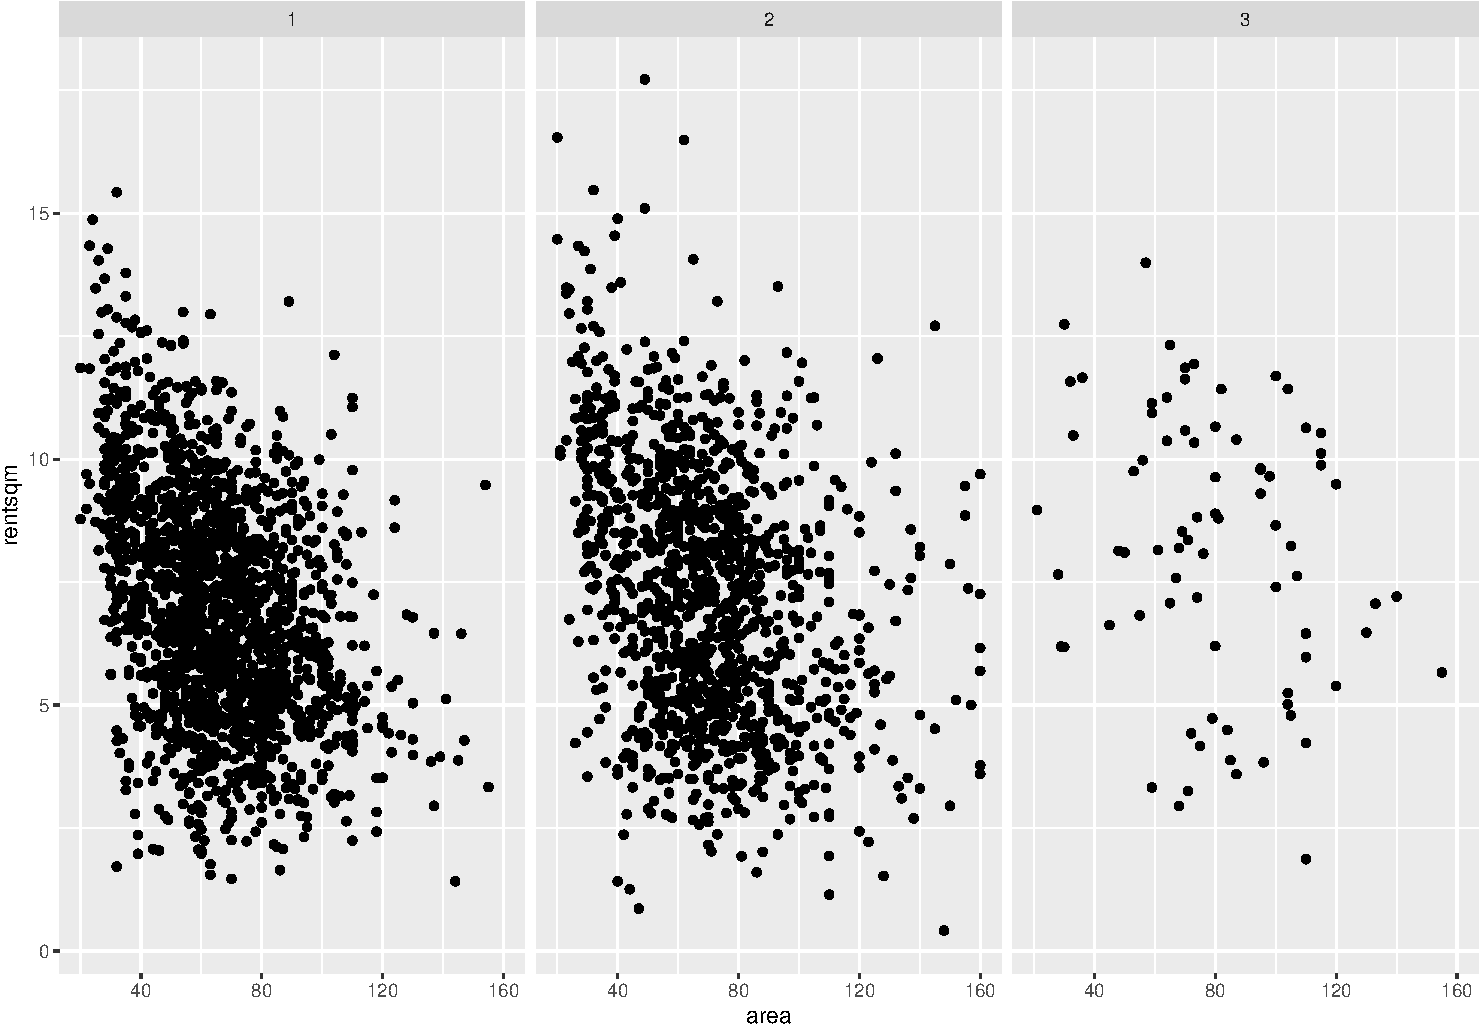
\includegraphics[keepaspectratio]{Module01IntroPresentation_files/figure-beamer/unnamed-chunk-4-1.pdf}}

\begin{Shaded}
\begin{Highlighting}[]
\FunctionTok{ggplot}\NormalTok{(}\AttributeTok{data =}\NormalTok{ ds, }\AttributeTok{mapping =} \FunctionTok{aes}\NormalTok{(}\AttributeTok{x =}\NormalTok{ location, }\AttributeTok{y =}\NormalTok{ rentsqm)) }\SpecialCharTok{+} 
  \FunctionTok{geom\_boxplot}\NormalTok{()}
\end{Highlighting}
\end{Shaded}

\pandocbounded{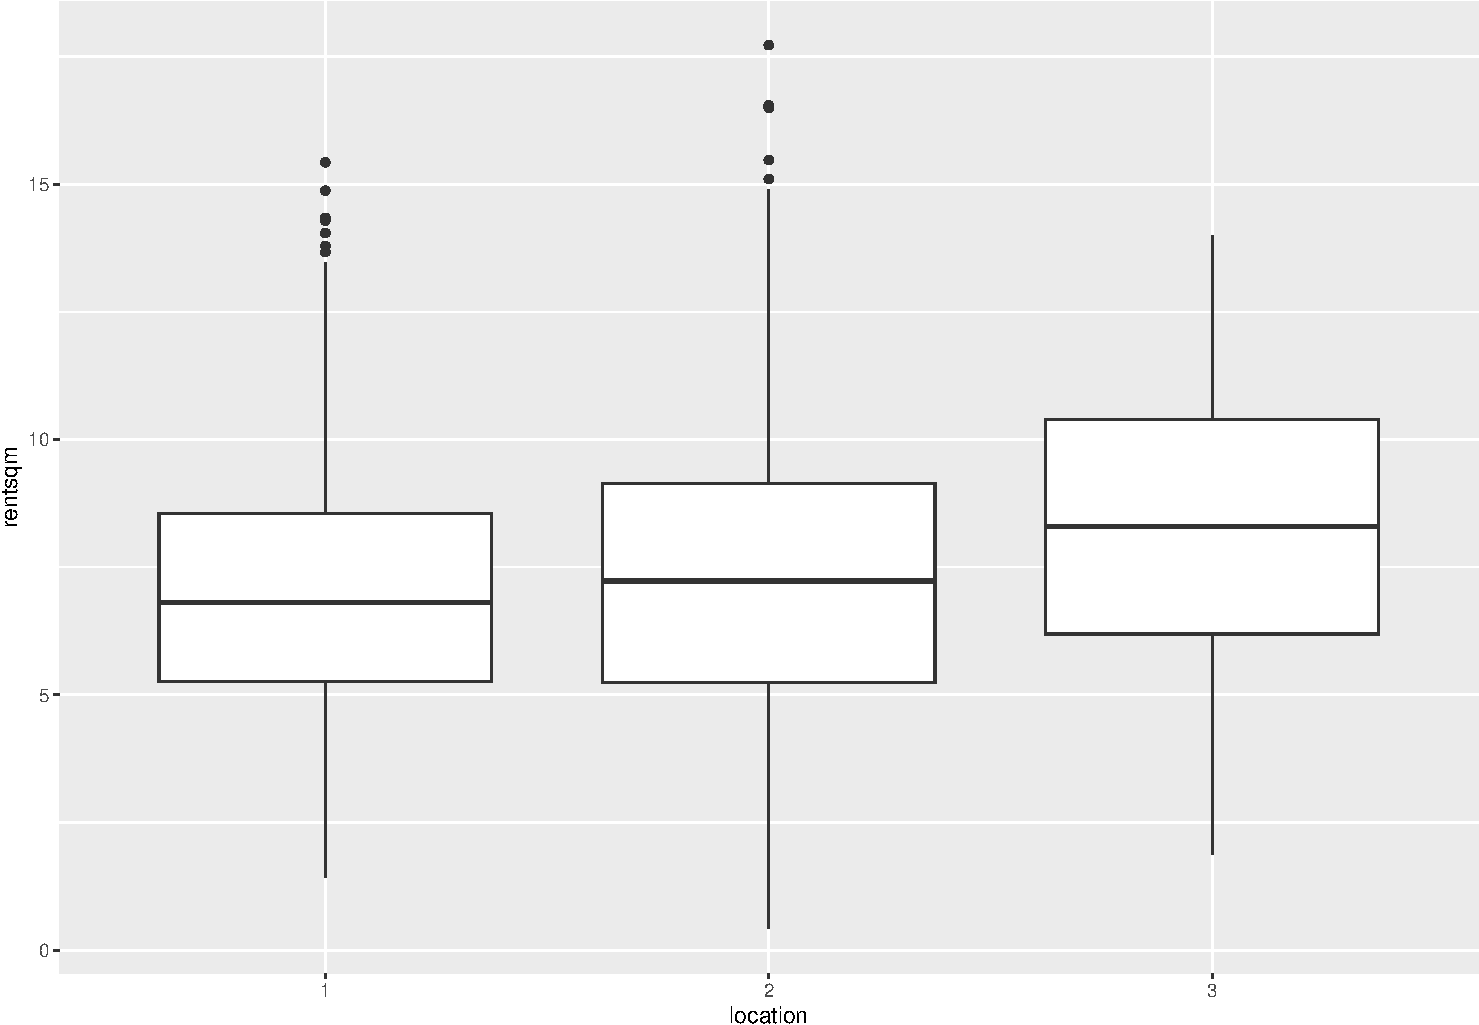
\includegraphics[keepaspectratio]{Module01IntroPresentation_files/figure-beamer/unnamed-chunk-4-2.pdf}}

So, location matters.

But, should we use \texttt{rent} or \texttt{rentsqm} as response?

\begin{Shaded}
\begin{Highlighting}[]
\FunctionTok{library}\NormalTok{(ggpubr)}
\end{Highlighting}
\end{Shaded}

\begin{verbatim}
## Warning: package 'ggpubr' was built under R version 4.5.1
\end{verbatim}

\begin{Shaded}
\begin{Highlighting}[]
\NormalTok{plot1 }\OtherTok{\textless{}{-}} \FunctionTok{ggplot}\NormalTok{(}\AttributeTok{data=}\NormalTok{ds) }\SpecialCharTok{+}
  \FunctionTok{geom\_density}\NormalTok{(}\AttributeTok{mapping=}\FunctionTok{aes}\NormalTok{(rent),}\AttributeTok{kernel=}\StringTok{"gaussian"}\NormalTok{)}
\NormalTok{plot2 }\OtherTok{\textless{}{-}} \FunctionTok{ggplot}\NormalTok{(}\AttributeTok{data=}\NormalTok{ds) }\SpecialCharTok{+}
  \FunctionTok{geom\_density}\NormalTok{(}\AttributeTok{mapping=}\FunctionTok{aes}\NormalTok{(rentsqm),}\AttributeTok{kernel=}\StringTok{"gaussian"}\NormalTok{)}
\FunctionTok{ggarrange}\NormalTok{(plot1, plot2, }\AttributeTok{ncol=}\DecValTok{2}\NormalTok{)}
\end{Highlighting}
\end{Shaded}

\pandocbounded{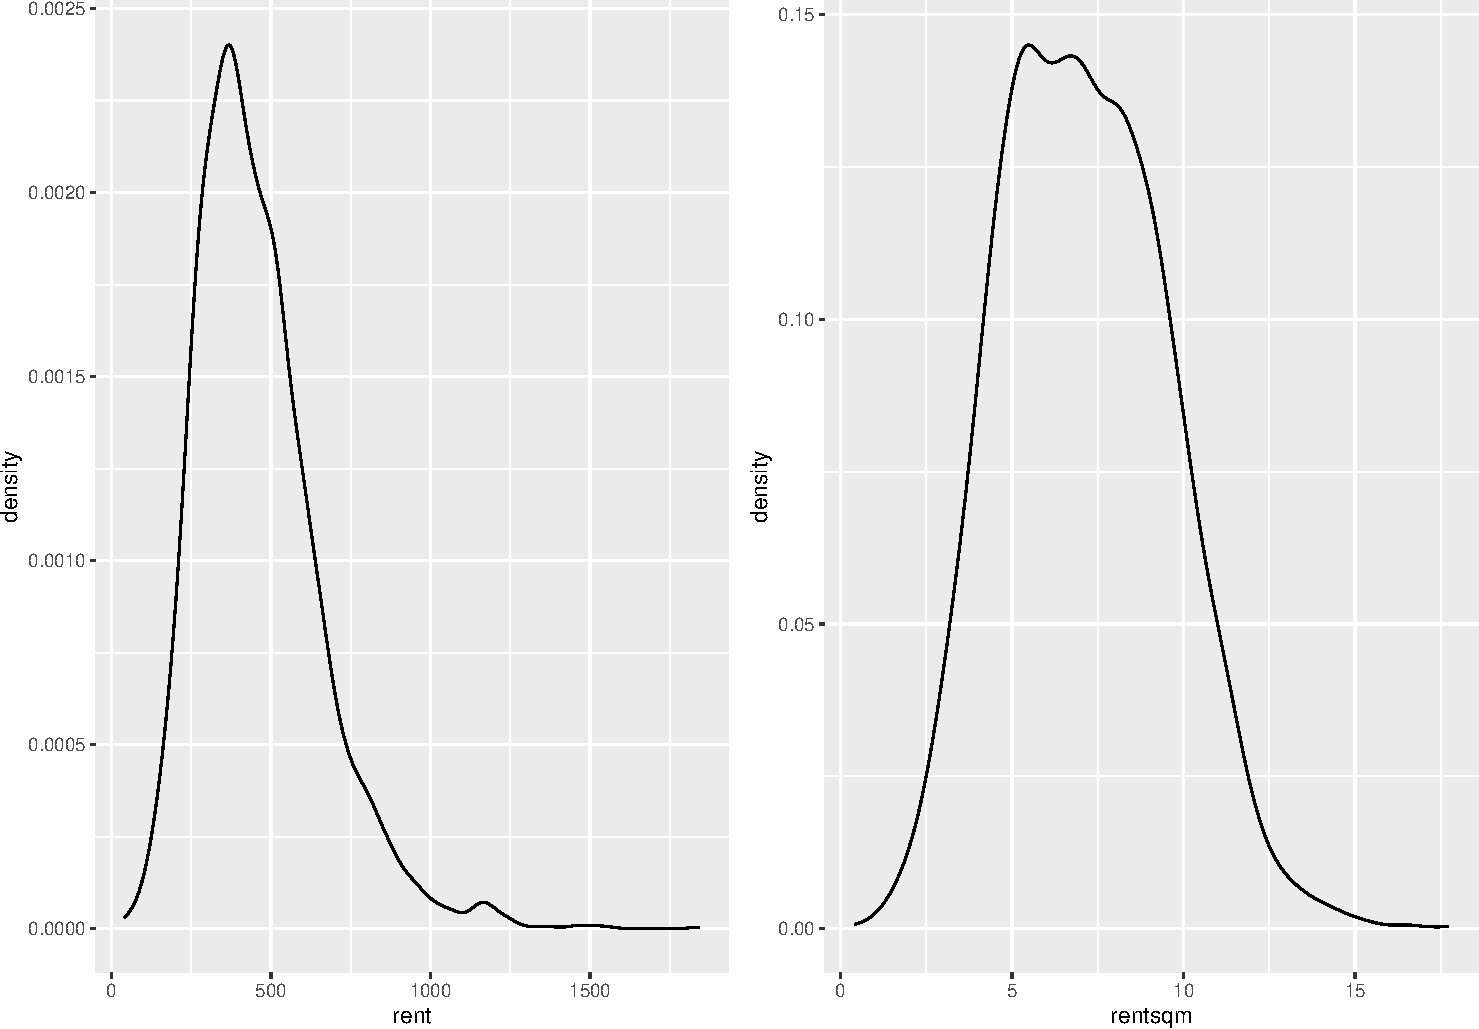
\includegraphics[keepaspectratio]{Module01IntroPresentation_files/figure-beamer/unnamed-chunk-5-1.pdf}}

So, which response will we use? And, what if we would include
\texttt{area} as covariate? I have plotted two plots together below,
more on mixing graphs on the same page (we need ggprbr, gridExtra and
cowplot packages)
\url{https://www.r-bloggers.com/ggplot2-easy-way-to-mix-multiple-graphs-on-the-same-page/}

Relationship between \texttt{rent} or \texttt{rentsqm} and \texttt{area}

\begin{Shaded}
\begin{Highlighting}[]
\NormalTok{plot1 }\OtherTok{\textless{}{-}} \FunctionTok{ggplot}\NormalTok{(}\AttributeTok{data=}\NormalTok{ds,}\FunctionTok{aes}\NormalTok{(area,rent))}\SpecialCharTok{+}
  \FunctionTok{geom\_point}\NormalTok{(}\AttributeTok{mapping=}\FunctionTok{aes}\NormalTok{(area,rent),}\AttributeTok{size=}\FloatTok{0.5}\NormalTok{)}
\NormalTok{plot2 }\OtherTok{\textless{}{-}} \FunctionTok{ggplot}\NormalTok{(}\AttributeTok{data=}\NormalTok{ds)}\SpecialCharTok{+}
  \FunctionTok{geom\_point}\NormalTok{(}\AttributeTok{mapping=}\FunctionTok{aes}\NormalTok{(area,rentsqm),}\AttributeTok{size=}\FloatTok{0.5}\NormalTok{)}
\FunctionTok{ggarrange}\NormalTok{(plot1, plot2, }\AttributeTok{ncol=}\DecValTok{2}\NormalTok{)}
\end{Highlighting}
\end{Shaded}

\pandocbounded{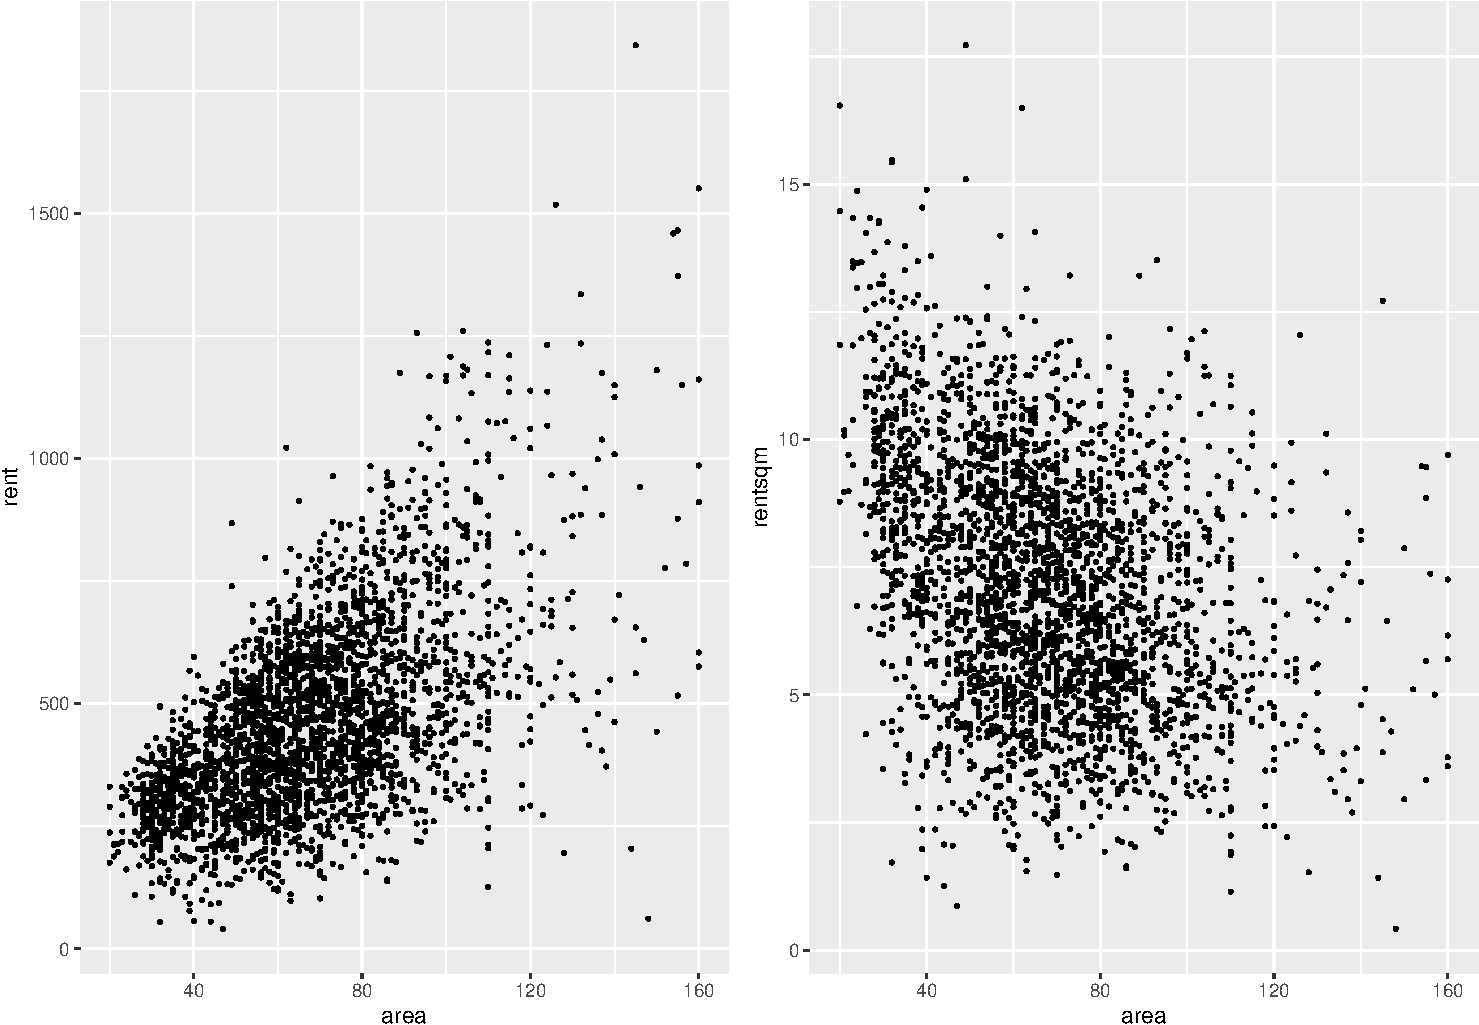
\includegraphics[keepaspectratio]{Module01IntroPresentation_files/figure-beamer/unnamed-chunk-6-1.pdf}}

So, if we include area as a covariate, we may look at residuals when
using \texttt{rent} or \texttt{rentsqm}. More about diagnostic plots in
Module 2 - but - which plot below looks more random?

\begin{Shaded}
\begin{Highlighting}[]
\NormalTok{lm.rent}\OtherTok{=}\FunctionTok{lm}\NormalTok{(rent}\SpecialCharTok{\textasciitilde{}}\NormalTok{area,}\AttributeTok{data=}\NormalTok{ds)}
\FunctionTok{summary}\NormalTok{(lm.rent)}
\end{Highlighting}
\end{Shaded}

\begin{verbatim}
## 
## Call:
## lm(formula = rent ~ area, data = ds)
## 
## Residuals:
##     Min      1Q  Median      3Q     Max 
## -786.63 -104.88   -5.69   95.93 1009.68 
## 
## Coefficients:
##             Estimate Std. Error t value Pr(>|t|)    
## (Intercept) 134.5922     8.6135   15.63   <2e-16 ***
## area          4.8215     0.1206   39.98   <2e-16 ***
## ---
## Signif. codes:  0 '***' 0.001 '**' 0.01 '*' 0.05 '.' 0.1 ' ' 1
## 
## Residual standard error: 158.8 on 3080 degrees of freedom
## Multiple R-squared:  0.3417, Adjusted R-squared:  0.3415 
## F-statistic:  1599 on 1 and 3080 DF,  p-value: < 2.2e-16
\end{verbatim}

\begin{Shaded}
\begin{Highlighting}[]
\NormalTok{lm.rentsqm}\OtherTok{=}\FunctionTok{lm}\NormalTok{(rentsqm}\SpecialCharTok{\textasciitilde{}}\NormalTok{area,}\AttributeTok{data=}\NormalTok{ds)}
\FunctionTok{summary}\NormalTok{(lm.rentsqm)}
\end{Highlighting}
\end{Shaded}

\begin{verbatim}
## 
## Call:
## lm(formula = rentsqm ~ area, data = ds)
## 
## Residuals:
##     Min      1Q  Median      3Q     Max 
## -6.9622 -1.5737 -0.1102  1.5861  9.9674 
## 
## Coefficients:
##             Estimate Std. Error t value Pr(>|t|)    
## (Intercept)  9.46883    0.12426   76.20   <2e-16 ***
## area        -0.03499    0.00174  -20.11   <2e-16 ***
## ---
## Signif. codes:  0 '***' 0.001 '**' 0.01 '*' 0.05 '.' 0.1 ' ' 1
## 
## Residual standard error: 2.291 on 3080 degrees of freedom
## Multiple R-squared:  0.1161, Adjusted R-squared:  0.1158 
## F-statistic: 404.5 on 1 and 3080 DF,  p-value: < 2.2e-16
\end{verbatim}

\begin{Shaded}
\begin{Highlighting}[]
\NormalTok{p1}\OtherTok{\textless{}{-}}\FunctionTok{ggplot}\NormalTok{(lm.rent, }\FunctionTok{aes}\NormalTok{(.fitted, .resid))}\SpecialCharTok{+}\FunctionTok{geom\_point}\NormalTok{()}
\NormalTok{p1}\OtherTok{\textless{}{-}}\NormalTok{p1}\SpecialCharTok{+}\FunctionTok{stat\_smooth}\NormalTok{(}\AttributeTok{method=}\StringTok{"loess"}\NormalTok{)}\SpecialCharTok{+}\FunctionTok{geom\_hline}\NormalTok{(}\AttributeTok{yintercept=}\DecValTok{0}\NormalTok{, }\AttributeTok{col=}\StringTok{"red"}\NormalTok{, }\AttributeTok{linetype=}\StringTok{"dashed"}\NormalTok{)}
\NormalTok{p1}\OtherTok{\textless{}{-}}\NormalTok{p1}\SpecialCharTok{+}\FunctionTok{xlab}\NormalTok{(}\StringTok{"Fitted values"}\NormalTok{)}\SpecialCharTok{+}\FunctionTok{ylab}\NormalTok{(}\StringTok{"Residuals"}\NormalTok{)}
\NormalTok{p1}\OtherTok{\textless{}{-}}\NormalTok{p1}\SpecialCharTok{+}\FunctionTok{ggtitle}\NormalTok{(}\StringTok{"Rent: Residual vs Fitted Plot"}\NormalTok{)}\SpecialCharTok{+}\FunctionTok{theme\_bw}\NormalTok{()}
\NormalTok{p2}\OtherTok{\textless{}{-}}\FunctionTok{ggplot}\NormalTok{(lm.rentsqm, }\FunctionTok{aes}\NormalTok{(.fitted, .resid))}\SpecialCharTok{+}\FunctionTok{geom\_point}\NormalTok{()}
\NormalTok{p2}\OtherTok{\textless{}{-}}\NormalTok{p2}\SpecialCharTok{+}\FunctionTok{stat\_smooth}\NormalTok{(}\AttributeTok{method=}\StringTok{"loess"}\NormalTok{)}\SpecialCharTok{+}\FunctionTok{geom\_hline}\NormalTok{(}\AttributeTok{yintercept=}\DecValTok{0}\NormalTok{, }\AttributeTok{col=}\StringTok{"red"}\NormalTok{, }\AttributeTok{linetype=}\StringTok{"dashed"}\NormalTok{)}
\NormalTok{p2}\OtherTok{\textless{}{-}}\NormalTok{p2}\SpecialCharTok{+}\FunctionTok{xlab}\NormalTok{(}\StringTok{"Fitted values"}\NormalTok{)}\SpecialCharTok{+}\FunctionTok{ylab}\NormalTok{(}\StringTok{"Residuals"}\NormalTok{)}
\NormalTok{p2}\OtherTok{\textless{}{-}}\NormalTok{p2}\SpecialCharTok{+}\FunctionTok{ggtitle}\NormalTok{(}\StringTok{"rentsqm: Residual vs Fitted Plot"}\NormalTok{)}\SpecialCharTok{+}\FunctionTok{theme\_bw}\NormalTok{()}
\FunctionTok{ggarrange}\NormalTok{(p1, p2, }\AttributeTok{ncol=}\DecValTok{2}\NormalTok{)}
\end{Highlighting}
\end{Shaded}

\begin{verbatim}
## `geom_smooth()` using formula = 'y ~ x'
## `geom_smooth()` using formula = 'y ~ x'
\end{verbatim}

\pandocbounded{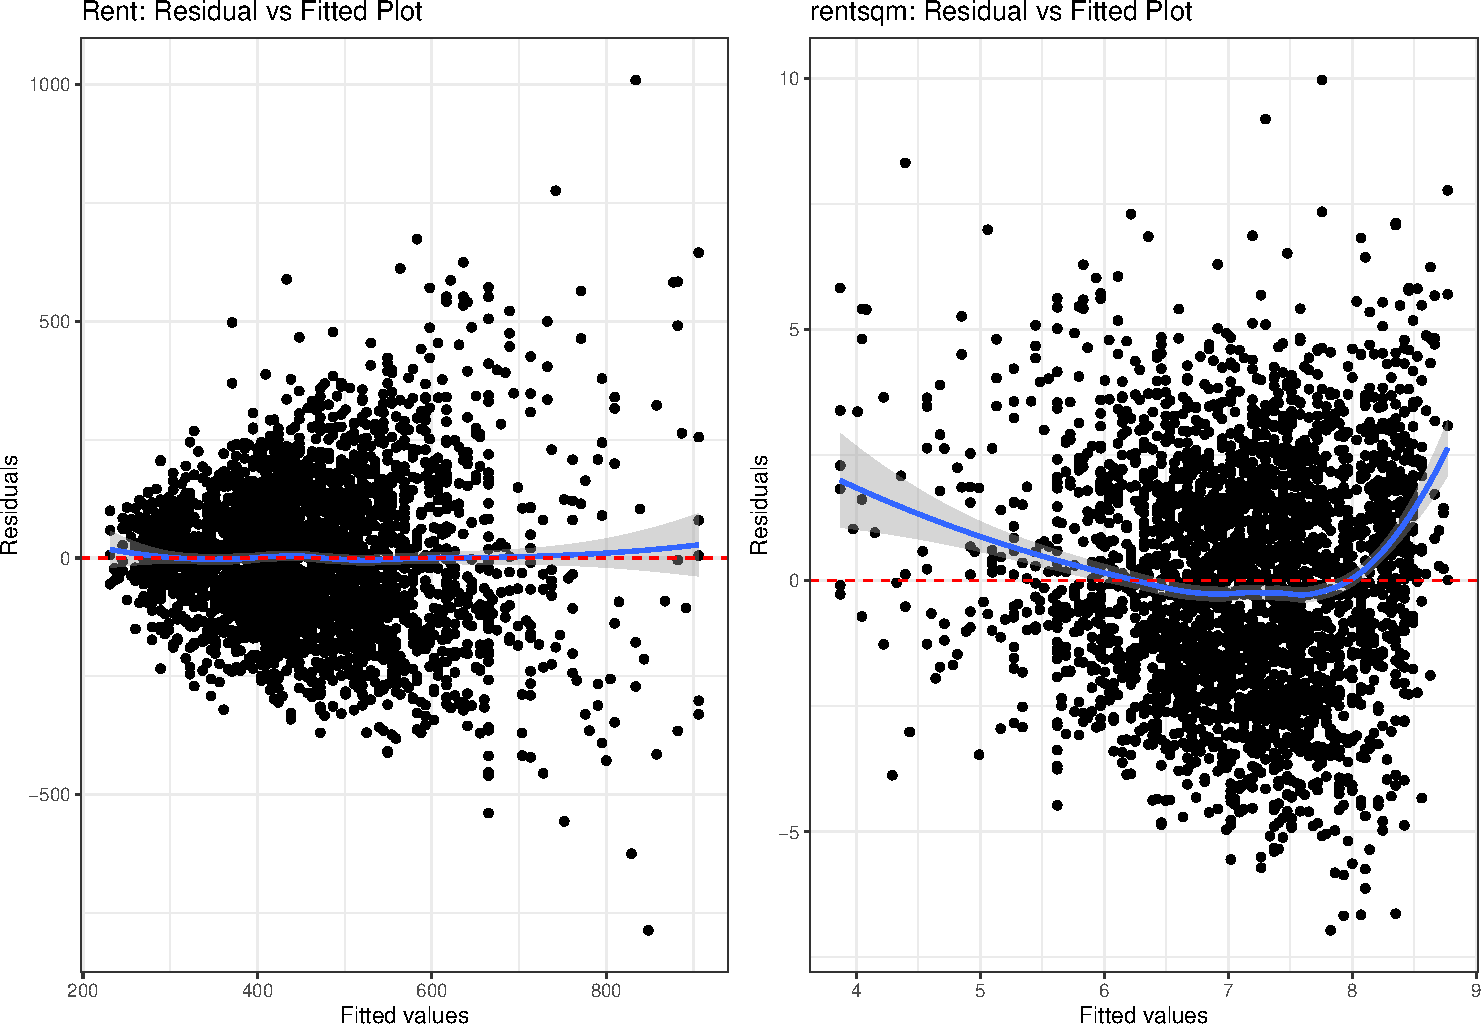
\includegraphics[keepaspectratio]{Module01IntroPresentation_files/figure-beamer/unnamed-chunk-7-1.pdf}}

Take home message: for the mean of the response may differ with out
covariates - that is why we use regression. For the normal linear
regression it is not the response that is supposed to have mean zero,
but the error term - more about this in Module 2. And, is the variance
of the residuals independent of the fitted values? Yes, more in Module
2.
\end{block}
\end{frame}

\begin{frame}
\begin{block}{Combining exercise 1 and 2:}
\phantomsection\label{combining-exercise-1-and-2}
Choose one of the distributions you studied earlier (binomial, Poisson,
normal or gamma), and write a R-markdown document answering the
questions on requirements, f(x), f(x) as exponential family and mean and
variance. Also add R-code to plot f(x) and F(x) for a given set of
parameters - and add the mean as a vertical line - using the ggplot
library. Submit your Rmd document to the lecturer (email) - so it can be
added to this module solutions, or make your own github repository and
email the link to your repo to be added to this module page.
\end{block}
\end{frame}

\begin{frame}{Further reading}
\phantomsection\label{further-reading}
\begin{itemize}
\item
  Grolemund and Hadwick (2017): ``R for Data Science'',
  \url{http://r4ds.had.co.nz}
\item
  Xie, Allaire and Grolemund (2018): ``R Markdown --- the definitive
  guide'', \url{https://bookdown.org/yihui/rmarkdown/}
\item
  Hadwick (2009):
  \href{https://link.springer.com/book/10.1007\%2F978-0-387-98141-3}{``ggplot2:
  Elegant graphics for data analysis'' textbook}.
\item
  Wilkinson (2005):
  \href{https://www.springer.com/gp/book/9780387245447}{The grammar of
  graphics}. The theory behind the ggplot2 package universe.
\item
  If you want to see more of the powers of ggplot, combined with a nice
  story:
  \url{https://www.andrewheiss.com/blog/2017/08/10/exploring-minards-1812-plot-with-ggplot2/}
\item
  R-bloggers: \url{https://https://www.r-bloggers.com/} is a good place
  to look for tutorials.
\item
  Stack Overflow: \url{https://stackoverflow.com/} is a good place to
  look for answers to your R questions (but also try the GLM teaching
  team)
\end{itemize}
\end{frame}

\end{document}
